\documentclass[titlepage=firstiscover, parskip=half, bibliography=totoc,captions=tableheading]{scrartcl} % KOMA-Script Dokumentenklasse Article

% Warnung, falls noch einmal kompiliert werden muss
\usepackage[aux]{rerunfilecheck}

% Paket für Schriftarteinstellung, muss immer geladen werden
\usepackage{fontspec}

% Deutsche Spracheinstellungen, wichtig z. B. für korrekte Trennung
\usepackage[ngerman]{babel}

% mehr Pakete hier
\usepackage{amsmath} % unverzichtbare Mathe-Befehle
\usepackage{amssymb} % viele Mathe-Symbole
\usepackage{mathtools} % Erweiterungen für amsmath
\usepackage[
math-style=ISO, % ┐
bold-style=ISO, % │
sans-style=italic, % │ ISO-Standard folgen
nabla=upright, % │
partial=upright, % │
mathrm=sym, % ┘
]{unicode-math}
\usepackage[
version=4,
math-greek=default,
text-greek=default,
]{mhchem}
\usepackage[section, below]{placeins}
\usepackage{caption} % Captions schöner machen
\usepackage{graphicx}
\usepackage{graphicx}
\usepackage{tabularray}
\usepackage[
locale=DE,
separate-uncertainty=true, % Immer Unsicherheit mit ±
per-mode=symbol-or-fraction, % m/s im Text, sonst \frac
% alternativ:
% per-mode=reciprocal, % m s^{-1}
% output-decimal-marker=., % . statt , für Dezimalzahlen
]{siunitx}

\UseTblrLibrary{booktabs}
\UseTblrLibrary{siunitx} % Lädt siunitx und definiert die S-Spalte
\usepackage[style=alphabetic]{biblatex} % nach babel
\addbibresource{lit.bib}

% Unterstützung für Links und PDF Metadaten
\usepackage[unicode]{hyperref}
\usepackage{bookmark}
\usepackage{microtype}
\usepackage{xfrac}
% Einstellungen hier, z.B. Fonts
\setmathfont{Latin Modern Math}
% \setmathfont{Tex Gyre Pagella Math} % alternativ




\begin{document}
\title{Das Hooksche Gesetz}
\author{
Sophia Brechmann \\
\texorpdfstring{\href{mailto:sophia.brechmann@tu-dortmund.de}{sophia.brechmann@tu-dortmund.de}\and}{,}
Simon Kugler \\
\texorpdfstring{\href{mailto:simon.kugler@tu-dortmund.de}{simon.kugler@tu-dortmund.de}}{}
}
\date{Deadline: Dienstag, 14.11.2023}
\maketitle
\tableofcontents
\newpage
\section{Ziel}
    In diesem Versuch wird die Federkonstante $D$ einer Feder bestimmt, in dem man diese auslenkt.
\section{Durchführung}
    Der Versuch wird online über die Seite der Uni Duisburg-Essen ausgeführt:\\
    http://kallisto.didaktik.physik.uni-due.de/IBEs/Hooke.php \\
    Eine vertikal aufgehangende Feder wird per Schnur über eine Umlenkrolle ausgelenkt. Das Ende der Schnur liegt an einem Lineal an, an welchem
    die Auslenkung $\Delta x$ abgetragen wird. An der Umlenkrolle wird die dafür benötigte Kraft $F$ in Newton $N$ gemessen und auf einem Laptop angezeigt.
\section{Auswertung}
    Folgende Messwerte wurden bestimmt:\\
    \begin{table}[h]
        \centering
        \caption{Messwerte des Versuchs "Hooksches Gesetz".}
        \label{tab:Messwerte}
        \begin{tblr}{colspec={c c c}}
            \toprule
            $\Delta x[\unit{\centi\meter}]$ & $F[\unit{\newton}]$ & $D[\unit{\newton\per\meter}]$ \\
            \midrule
            2,5 $\pm 0,5$ & 0,07$\pm 0,01$ & 2,800\\
            4,5 $\pm 0,5$ & 0,13$\pm 0,01$ & 2,889\\
            9,0 $\pm 0,5$ & 0,27$\pm 0,01$ & 3,000\\ 
            13,5$\pm 0,5$ & 0,39$\pm 0,01$ & 2,889\\
            21,0$\pm 0,5$ & 0,62$\pm 0,01$ & 2,952\\
            23,5$\pm 0,5$ & 0,69$\pm 0,01$ & 2,936\\
            29,0$\pm 0,5$ & 0,86$\pm 0,01$ & 2,966\\
            34,5$\pm 0,5$ & 1,03$\pm 0,01$ & 2,986\\
            38,0$\pm 0,5$ & 1,13$\pm 0,01$ & 2,974\\
            42,5$\pm 0,5$ & 1,26$\pm 0,01$ & 2,965\\
            \bottomrule
        \end{tblr}
    \end{table}
\\
Berechnet man aus den 10 bzw. 20 Werten jeweils über die Beziehung $D=\frac{F}{\Delta x}$ die Federkonstante
und berechnet daraus den Mittelwert, ergibt sich: $\overline{D}=29,357\unit{\newton\per\meter}$.\\
Mit Fehlerrechnung erhält man folgende Abweichung für $D$: \\
\begin{align*}
    \Delta D&=\sqrt{(\frac{d}{dF}(\frac{F}{\Delta x}))^2\cdot(\Delta F)^2+(\frac{d}{d\Delta x}(\frac{F}{\Delta x}))^2(\Delta(\Delta x))^2}\\
    &=\sqrt{\frac{1}{(0,218\unit{\meter})^2}\cdot (0,01\unit{\newton})^2+(-\frac{6,18\unit{\newton}}{(0,218\unit{m})^2})^2\cdot(0,005\unit{m})^2}\\
    &=\num{0,65}\unit{\newton\per\meter}\\
    % \Rightarrow D&=(29,36\pm 6,52\cdot10^{-3})\unit{N/m}\\
    \Rightarrow D&=(2,936\pm\num{0.65})\unit{\newton\per\meter}
\end{align*}
\newpage
Nun wird die Federkonstante $D$ mithilfe einer linearen Regression berechnet. Graphisch sieht eine durch die Messwerte gelegte lineare Funktion wie folgt aus:
\begin{figure}[h]
    \centering
    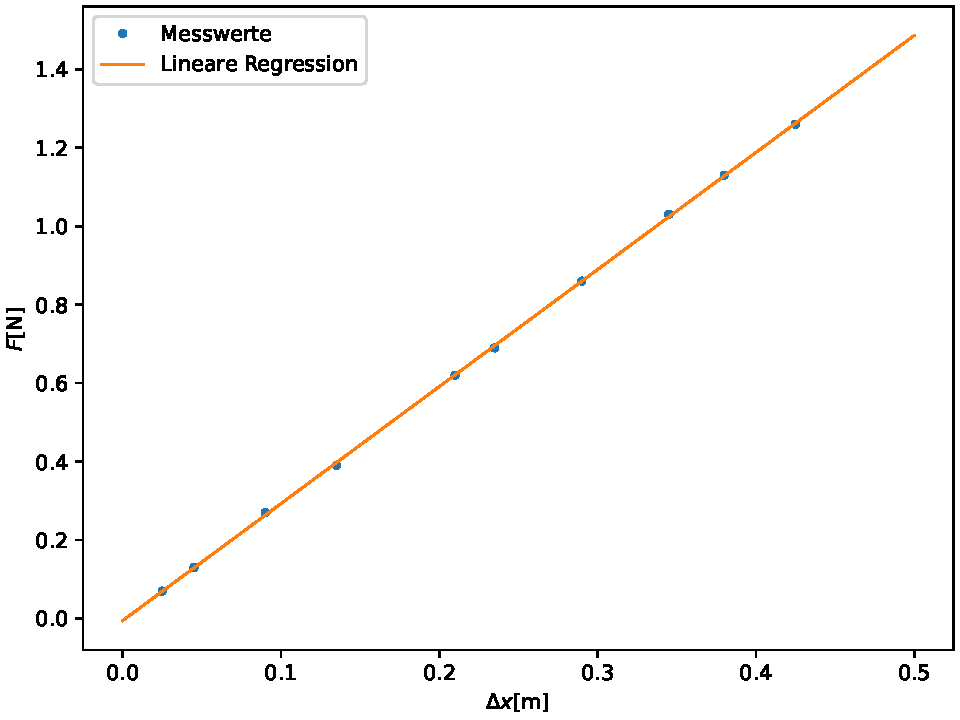
\includegraphics[width=\textwidth]{Linreg.pdf}
    \label{Lineare Regression der Messwerte.}
\end{figure}\\
Mittels Python lassen sich die Koeffizienten, welche zur Bestimmung einer Funktion der Form $g(x)=ax+b$ von nöten sind, bestimmen:\\
\begin{align*}
a&=2,982\pm0,011\\
b&=-0,005\pm0,003\\
\intertext{Die Gerade wird also durch die Vorschrift $g(x)=(2,982\pm0,01)x-0,005$ beschrieben.
Die Steigung entspricht unserer Federkonstante, genau dem Verhältnis zwischen $\Delta x$ und F. Der y-Achsenabschnitt müsste eigentlich im Nullpunkt liegen, 
jedoch kommt hier durch Messunsicherheiten die Abweichung zustande. 
So kann die Federkonstante genauer bestimmt werden.
Damit ist:}
D&=(2,98\pm0,01)\unit{\newton\per\meter}
\end{align*}
\\
\newpage
Da wir uns nicht sicher waren, welcher Weg genau mit "linearer Ausgleichsrechnung" gemeint ist, haben wir auch noch folgende - die Methode der kleinen Quadrate - verwendet:\\
Hierbei ist $\vec r$ der Residuenvektor, $\vec{\Delta x}$ die Ansammlung unserer Messwerte in einem und $\vec C$ der Vektor für die Kraftmesswerte. $D$ wird dann durch $x$ dargestellt.\\
Es gilt: $\vec r= D\cdot\vec{\Delta x}-\vec F$, außerdem $A^T\cdot A\cdot x=A^T\cdot\vec C$.
\begin{align*}
    \Rightarrow (\vec{\Delta x})^T\cdot(\vec{\Delta x})\cdot x&=(\vec{\Delta x})^T\cdot\vec C 
    \intertext{ergibt mit eingesetzten Werten und den daraus resultierenden Skalarprodukten:}
    6564,5\unit{\centi\meter\squared}\cdot x&=194,655\unit[inter-unit-product=\cdot]{\centi\meter\newton}\\
    \Leftrightarrow x&=2,97\unit{\newton\per\meter}
\end{align*}
Da wir uns nicht sicher waren, wie man bei Skalarprodukten den Fehler berechnet (evtl. eine Summe über die Fehler jeder Zeile/Spalte?), haben wir die 
Fehllerrechnung hier ausgelassen.
\end{document}